%% bare_conf.tex
%% V1.3
%% 2007/01/11
%% by Michael Shell
%% See:
%% http://www.michaelshell.org/
%% for current contact information.
%%
%% This is a skeleton file demonstrating the use of IEEEtran.cls
%% (requires IEEEtran.cls version 1.7 or later) with an IEEE conference paper.
%%
%% Support sites:
%% http://www.michaelshell.org/tex/ieeetran/
%% http://www.ctan.org/tex-archive/macros/latex/contrib/IEEEtran/
%% and
%% http://www.ieee.org/

%%*************************************************************************
%% Legal Notice:
%% This code is offered as-is without any warranty either expressed or
%% implied; without even the implied warranty of MERCHANTABILITY or
%% FITNESS FOR A PARTICULAR PURPOSE! 
%% User assumes all risk.
%% In no event shall IEEE or any contributor to this code be liable for
%% any damages or losses, including, but not limited to, incidental,
%% consequential, or any other damages, resulting from the use or misuse
%% of any information contained here.
%%
%% All comments are the opinions of their respective authors and are not
%% necessarily endorsed by the IEEE.
%%
%% This work is distributed under the LaTeX Project Public License (LPPL)
%% ( http://www.latex-project.org/ ) version 1.3, and may be freely used,
%% distributed and modified. A copy of the LPPL, version 1.3, is included
%% in the base LaTeX documentation of all distributions of LaTeX released
%% 2003/12/01 or later.
%% Retain all contribution notices and credits.
%% ** Modified files should be clearly indicated as such, including  **
%% ** renaming them and changing author support contact information. **
%%
%% File list of work: IEEEtran.cls, IEEEtran_HOWTO.pdf, bare_adv.tex,
%%                    bare_conf.tex, bare_jrnl.tex, bare_jrnl_compsoc.tex
%%*************************************************************************

% *** Authors should verify (and, if needed, correct) their LaTeX system  ***
% *** with the testflow diagnostic prior to trusting their LaTeX platform ***
% *** with production work. IEEE's font choices can trigger bugs that do  ***
% *** not appear when using other class files.                            ***
% The testflow support page is at:
% http://www.michaelshell.org/tex/testflow/



% Note that the a4paper option is mainly intended so that authors in
% countries using A4 can easily print to A4 and see how their papers will
% look in print - the typesetting of the document will not typically be
% affected with changes in paper size (but the bottom and side margins will).
% Use the testflow package mentioned above to verify correct handling of
% both paper sizes by the user's LaTeX system.
%
% Also note that the "draftcls" or "draftclsnofoot", not "draft", option
% should be used if it is desired that the figures are to be displayed in
% draft mode.
%
\documentclass[conference]{IEEEtran}
% Add the compsoc option for Computer Society conferences.
%
% If IEEEtran.cls has not been installed into the LaTeX system files,
% manually specify the path to it like:
% \documentclass[conference]{../sty/IEEEtran}





% Some very useful LaTeX packages include:
% (uncomment the ones you want to load)


% *** MISC UTILITY PACKAGES ***
%\usepackage{includegraphics}
%\usepackage{ifpdf}
% Heiko Oberdiek's ifpdf.sty is very useful if you need conditional
% compilation based on whether the output is pdf or dvi.
% usage:
% \ifpdf
%   % pdf code
% \else
%   % dvi code
% \fi
% The latest version of ifpdf.sty can be obtained from:
% http://www.ctan.org/tex-archive/macros/latex/contrib/oberdiek/
% Also, note that IEEEtran.cls V1.7 and later provides a builtin
% \ifCLASSINFOpdf conditional that works the same way.
% When switching from latex to pdflatex and vice-versa, the compiler may
% have to be run twice to clear warning/error messages.






% *** CITATION PACKAGES ***
%
%\usepackage{cite}
% cite.sty was written by Donald Arseneau
% V1.6 and later of IEEEtran pre-defines the format of the cite.sty package
% \cite{} output to follow that of IEEE. Loading the cite package will
% result in citation numbers being automatically sorted and properly
% "compressed/ranged". e.g., [1], [9], [2], [7], [5], [6] without using
% cite.sty will become [1], [2], [5]--[7], [9] using cite.sty. cite.sty's
% \cite will automatically add leading space, if needed. Use cite.sty's
% noadjust option (cite.sty V3.8 and later) if you want to turn this off.
% cite.sty is already installed on most LaTeX systems. Be sure and use
% version 4.0 (2003-05-27) and later if using hyperref.sty. cite.sty does
% not currently provide for hyperlinked citations.
% The latest version can be obtained at:
% http://www.ctan.org/tex-archive/macros/latex/contrib/cite/
% The documentation is contained in the cite.sty file itself.






% *** GRAPHICS RELATED PACKAGES ***
%
\ifCLASSINFOpdf
   \usepackage[pdftex]{graphicx}
  % declare the path(s) where your graphic files are
  % \graphicspath{{../pdf/}{../jpeg/}}
  % and their extensions so you won't have to specify these with
  % every instance of \includegraphics
  % \DeclareGraphicsExtensions{.pdf,.jpeg,.png}
\else
  % or other class option (dvipsone, dvipdf, if not using dvips). graphicx
  % will default to the driver specified in the system graphics.cfg if no
  % driver is specified.
  % \usepackage[dvips]{graphicx}
  % declare the path(s) where your graphic files are
  % \graphicspath{{../eps/}}
  % and their extensions so you won't have to specify these with
  % every instance of \includegraphics
  % \DeclareGraphicsExtensions{.eps}
\fi
% graphicx was written by David Carlisle and Sebastian Rahtz. It is
% required if you want graphics, photos, etc. graphicx.sty is already
% installed on most LaTeX systems. The latest version and documentation can
% be obtained at: 
% http://www.ctan.org/tex-archive/macros/latex/required/graphics/
% Another good source of documentation is "Using Imported Graphics in
% LaTeX2e" by Keith Reckdahl which can be found as epslatex.ps or
% epslatex.pdf at: http://www.ctan.org/tex-archive/info/
%
% latex, and pdflatex in dvi mode, support graphics in encapsulated
% postscript (.eps) format. pdflatex in pdf mode supports graphics
% in .pdf, .jpeg, .png and .mps (metapost) formats. Users should ensure
% that all non-photo figures use a vector format (.eps, .pdf, .mps) and
% not a bitmapped formats (.jpeg, .png). IEEE frowns on bitmapped formats
% which can result in "jaggedy"/blurry rendering of lines and letters as
% well as large increases in file sizes.
%
% You can find documentation about the pdfTeX application at:
% http://www.tug.org/applications/pdftex





% *** MATH PACKAGES ***
%
%\usepackage[cmex10]{amsmath}
% A popular package from the American Mathematical Society that provides
% many useful and powerful commands for dealing with mathematics. If using
% it, be sure to load this package with the cmex10 option to ensure that
% only type 1 fonts will utilized at all point sizes. Without this option,
% it is possible that some math symbols, particularly those within
% footnotes, will be rendered in bitmap form which will result in a
% document that can not be IEEE Xplore compliant!
%
% Also, note that the amsmath package sets \interdisplaylinepenalty to 10000
% thus preventing page breaks from occurring within multiline equations. Use:
%\interdisplaylinepenalty=2500
% after loading amsmath to restore such page breaks as IEEEtran.cls normally
% does. amsmath.sty is already installed on most LaTeX systems. The latest
% version and documentation can be obtained at:
% http://www.ctan.org/tex-archive/macros/latex/required/amslatex/math/





% *** SPECIALIZED LIST PACKAGES ***
%
%\usepackage{algorithmic}
% algorithmic.sty was written by Peter Williams and Rogerio Brito.
% This package provides an algorithmic environment fo describing algorithms.
% You can use the algorithmic environment in-text or within a figure
% environment to provide for a floating algorithm. Do NOT use the algorithm
% floating environment provided by algorithm.sty (by the same authors) or
% algorithm2e.sty (by Christophe Fiorio) as IEEE does not use dedicated
% algorithm float types and packages that provide these will not provide
% correct IEEE style captions. The latest version and documentation of
% algorithmic.sty can be obtained at:
% http://www.ctan.org/tex-archive/macros/latex/contrib/algorithms/
% There is also a support site at:
% http://algorithms.berlios.de/index.html
% Also of interest may be the (relatively newer and more customizable)
% algorithmicx.sty package by Szasz Janos:
% http://www.ctan.org/tex-archive/macros/latex/contrib/algorithmicx/




% *** ALIGNMENT PACKAGES ***
%
%\usepackage{array}
% Frank Mittelbach's and David Carlisle's array.sty patches and improves
% the standard LaTeX2e array and tabular environments to provide better
% appearance and additional user controls. As the default LaTeX2e table
% generation code is lacking to the point of almost being broken with
% respect to the quality of the end results, all users are strongly
% advised to use an enhanced (at the very least that provided by array.sty)
% set of table tools. array.sty is already installed on most systems. The
% latest version and documentation can be obtained at:
% http://www.ctan.org/tex-archive/macros/latex/required/tools/


%\usepackage{mdwmath}
%\usepackage{mdwtab}
% Also highly recommended is Mark Wooding's extremely powerful MDW tools,
% especially mdwmath.sty and mdwtab.sty which are used to format equations
% and tables, respectively. The MDWtools set is already installed on most
% LaTeX systems. The lastest version and documentation is available at:
% http://www.ctan.org/tex-archive/macros/latex/contrib/mdwtools/


% IEEEtran contains the IEEEeqnarray family of commands that can be used to
% generate multiline equations as well as matrices, tables, etc., of high
% quality.


%\usepackage{eqparbox}
% Also of notable interest is Scott Pakin's eqparbox package for creating
% (automatically sized) equal width boxes - aka "natural width parboxes".
% Available at:
% http://www.ctan.org/tex-archive/macros/latex/contrib/eqparbox/





% *** SUBFIGURE PACKAGES ***
%\usepackage[tight,footnotesize]{subfigure}
% subfigure.sty was written by Steven Douglas Cochran. This package makes it
% easy to put subfigures in your figures. e.g., "Figure 1a and 1b". For IEEE
% work, it is a good idea to load it with the tight package option to reduce
% the amount of white space around the subfigures. subfigure.sty is already
% installed on most LaTeX systems. The latest version and documentation can
% be obtained at:
% http://www.ctan.org/tex-archive/obsolete/macros/latex/contrib/subfigure/
% subfigure.sty has been superceeded by subfig.sty.



%\usepackage[caption=false]{caption}
%\usepackage[font=footnotesize]{subfig}
% subfig.sty, also written by Steven Douglas Cochran, is the modern
% replacement for subfigure.sty. However, subfig.sty requires and
% automatically loads Axel Sommerfeldt's caption.sty which will override
% IEEEtran.cls handling of captions and this will result in nonIEEE style
% figure/table captions. To prevent this problem, be sure and preload
% caption.sty with its "caption=false" package option. This is will preserve
% IEEEtran.cls handing of captions. Version 1.3 (2005/06/28) and later 
% (recommended due to many improvements over 1.2) of subfig.sty supports
% the caption=false option directly:
%\usepackage[caption=false,font=footnotesize]{subfig}
%
% The latest version and documentation can be obtained at:
% http://www.ctan.org/tex-archive/macros/latex/contrib/subfig/
% The latest version and documentation of caption.sty can be obtained at:
% http://www.ctan.org/tex-archive/macros/latex/contrib/caption/




% *** FLOAT PACKAGES ***
%
%\usepackage{fixltx2e}
% fixltx2e, the successor to the earlier fix2col.sty, was written by
% Frank Mittelbach and David Carlisle. This package corrects a few problems
% in the LaTeX2e kernel, the most notable of which is that in current
% LaTeX2e releases, the ordering of single and double column floats is not
% guaranteed to be preserved. Thus, an unpatched LaTeX2e can allow a
% single column figure to be placed prior to an earlier double column
% figure. The latest version and documentation can be found at:
% http://www.ctan.org/tex-archive/macros/latex/base/



%\usepackage{stfloats}
% stfloats.sty was written by Sigitas Tolusis. This package gives LaTeX2e
% the ability to do double column floats at the bottom of the page as well
% as the top. (e.g., "\begin{figure*}[!b]" is not normally possible in
% LaTeX2e). It also provides a command:
%\fnbelowfloat
% to enable the placement of footnotes below bottom floats (the standard
% LaTeX2e kernel puts them above bottom floats). This is an invasive package
% which rewrites many portions of the LaTeX2e float routines. It may not work
% with other packages that modify the LaTeX2e float routines. The latest
% version and documentation can be obtained at:
% http://www.ctan.org/tex-archive/macros/latex/contrib/sttools/
% Documentation is contained in the stfloats.sty comments as well as in the
% presfull.pdf file. Do not use the stfloats baselinefloat ability as IEEE
% does not allow \baselineskip to stretch. Authors submitting work to the
% IEEE should note that IEEE rarely uses double column equations and
% that authors should try to avoid such use. Do not be tempted to use the
% cuted.sty or midfloat.sty packages (also by Sigitas Tolusis) as IEEE does
% not format its papers in such ways.





% *** PDF, URL AND HYPERLINK PACKAGES ***
%
%\usepackage{url}
% url.sty was written by Donald Arseneau. It provides better support for
% handling and breaking URLs. url.sty is already installed on most LaTeX
% systems. The latest version can be obtained at:
% http://www.ctan.org/tex-archive/macros/latex/contrib/misc/
% Read the url.sty source comments for usage information. Basically,
% \url{my_url_here}.





% *** Do not adjust lengths that control margins, column widths, etc. ***
% *** Do not use packages that alter fonts (such as pslatex).         ***
% There should be no need to do such things with IEEEtran.cls V1.6 and later.
% (Unless specifically asked to do so by the journal or conference you plan
% to submit to, of course. )
\usepackage{mathtools}

% correct bad hyphenation here
\hyphenation{op-tical net-works semi-conduc-tor}


\begin{document}
%
% paper title
% can use linebreaks \\ within to get better formatting as desired
\title{Automated Generation of Search-able PDF Format of Chemical Equations from Document Images}


% author names and affiliations
% use a multiple column layout for up to three different
% affiliations
\author{\IEEEauthorblockN{Prerana Jana, Anubhab Majumdar, Sekhar Mandal}
\IEEEauthorblockA{Department of Computer Science and Technology\\
Indian Institute of Engineer Science and Technology\\
Shibpur, India\\
Email: (prerana.jana, anubhabmajumdar93)@gmail.com\\sekhar@cs.iiests.ac.in}
\and
\IEEEauthorblockN{Bhabatosh Chanda}
\IEEEauthorblockA{Electronics and Communication Sciences Unit\\
Indian Statistical Institute\\ Kolkata, India\\
Email: chanda@isical.ac.in}}
%\and
%\IEEEauthorblockN{James Kirk\\ and Montgomery Scott}
%\IEEEauthorblockA{Starfleet Academy\\
%San Francisco, California 96678-2391\\
%Telephone: (800) 555--1212\\
%Fax: (888) 555--1212}}

% conference papers do not typically use \thanks and this command
% is locked out in conference mode. If really needed, such as for
% the acknowledgment of grants, issue a \IEEEoverridecommandlockouts
% after \documentclass

% for over three affiliations, or if they all won't fit within the width
% of the page, use this alternative format:
% 
%\author{\IEEEauthorblockN{Michael Shell\IEEEauthorrefmark{1},
%Homer Simpson\IEEEauthorrefmark{2},
%James Kirk\IEEEauthorrefmark{3}, 
%Montgomery Scott\IEEEauthorrefmark{3} and
%Eldon Tyrell\IEEEauthorrefmark{4}}
%\IEEEauthorblockA{\IEEEauthorrefmark{1}School of Electrical and Computer Engineering\\
%Georgia Institute of Technology,
%Atlanta, Georgia 30332--0250\\ Email: see http://www.michaelshell.org/contact.html}
%\IEEEauthorblockA{\IEEEauthorrefmark{2}Twentieth Century Fox, Springfield, USA\\
%Email: homer@thesimpsons.com}
%\IEEEauthorblockA{\IEEEauthorrefmark{3}Starfleet Academy, San Francisco, California 96678-2391\\
%Telephone: (800) 555--1212, Fax: (888) 555--1212}
%\IEEEauthorblockA{\IEEEauthorrefmark{4}Tyrell Inc., 123 Replicant Street, Los Angeles, California 90210--4321}}




% use for special paper notices
%\IEEEspecialpapernotice{(Invited Paper)}




% make the title area
\maketitle


\begin{abstract}
%\boldmath
%Segmentation of mathematical equations from document images is already a major research area for improved performance of OCR systems. Though chemical equations are
%also sharing similar spatial properties as that of mathematical equations, efforts to segment those are still to be explored. This paper presents a method for segmenting and detecting chemical  in heterogeneous document images that may
%contain graphics, tables, text, chemical and non-chemical equations. Finally, the detected chemical equation is converted into searchable PDF format. In our proposed method we extracted the equations using morphological operators and histogram
%analysis and the extracted equations are detected  using MATLAB R2014a OCR engine.
%The proposed method is tested on 240 document images and experimental results are encouraging.
PDF format of scanned document images is not searchable. OCR tries to remedy this adversity by converting images or PDF files into editable and searchable data, but it has it’s own limitations in presence of equations - both mathematical and chemical.  OCR system for mathematical document images is already a major research area and has provided successful result. However, chemical equation segmentation has been a less 
ventured road. In this paper we present a novel method for automated generation of searchable PDF format of segmented chemical equations from scanned document images  by performing chemical symbol recognition and auto-correction of chemical reactants.  We use existing OCR systems, pattern recognition, contextual data analysis and a standard \LaTeX\  package to generate the chemical equation in searchable PDF format.
The effectiveness of the proposed method is demonstrated by testing it on 240 document images.
%Index Terms— Grayscale morphological operations, Background estimation. Histogram analysis

\keywords Chemical equations, mathematical symbols, morphological operation.
\end{abstract}
% IEEEtran.cls defaults to using nonbold math in the Abstract.
% This preserves the distinction between vectors and scalars. However,
% if the conference you are submitting to favors bold math in the abstract,
% then you can use LaTeX's standard command \boldmath at the very start
% of the abstract to achieve this. Many IEEE journals/conferences frown on
% math in the abstract anyway.

% no keywords%




% For peer review papers, you can put extra information on the cover
% page as needed:
% \ifCLASSOPTIONpeerreview
% \begin{center} \bfseries EDICS Category: 3-BBND \end{center}
% \fi
%
% For peerreview papers, this IEEEtran command inserts a page break and
% creates the second title. It will be ignored for other modes.
\IEEEpeerreviewmaketitle



\section{Introduction}
We use search engines like Google to find location of documents in WWW. Usually, text-based keywords are used for retrieving of documents. 
A large number of documents are being digitized today for the purpose of archival analysis, transmission and browsing. The existing OCR systems show high accuracy in interpreting text portions, but fail to properly process other components
like graphics, half-tones, chemical and mathematical equations.

A few studies~\cite{blostein_97},~\cite{chan_00},~\cite{Garain_07} are directed toward math-symbol or math equation recognition assuming that the math-zones
are already marked. In~\cite{uchid_10} Fujiyoshi et al. proposed  a formal grammar for the verification of mathematical formulae for a practical mathematical OCR system.
We, on the other hand, contend that a better approach is to segment the chemical equations from the mixed material thereby helping the future OCR activity to focus it’s processing only on specific content. In this paper we propose  fully automated segmentation and detection technique of chemical equations
present in heterogeneous document images followed by generation of \LaTeX\ file of the segmented equations.

There are some methods that are used to reconstruct chemical molecules form scanned imge. They have used chemical datasets. Algorri et al.~\cite{algorri_07, algorri_07a} proposed a system that reconstruct chemical molecules from scanned document. They have used connected component analysis and their own vectorisation algorithm for character recognition. Connected components that are not recognised by the OCR engine, are used to produce a graph of vectors. A rule based approach reconstructs the molecule description from the vector graph and the character information. 
ChemReader~\cite{park_09} starts with connected component. Alphanumerics are  recognised using using the GOCR open source OCR tool. Graphical components are  identified using Hough transforms, corner detection and other bespoke algorithms.

% no \IEEEPARstart
%A lot of initiative is taken now, both in academia and industry,  not only to archive the historical documents, but also processing the same for classifying, indexing, 
%searching, extraction of text and images, contents based retrieval, etc.\@  
%for dissemination of this wealth of information on human history across the globe. 
%The first task towards the processing of the documents  starts usually  with binarization of the scanned image as a 
%pre-processing step. The objective of the binarization is to clearly divide the pixels into two classes, namely, 
%the foreground and the background.   The accuracy of binarization  is pivotal for the  success of the subsequent steps for further processing. 
%Handwritten documents, particularly the historical documents are difficult to binarize due to lack of
%standardization of the input and degradation of all sorts due to ageing and  other factors. 
%In historical handwritten documents the degradation includes
%faint characters, bleeding through and ink stains. Some
%noise may  also be introduced in the scanning process in the form of   black patches or back impressions.
%Figure  \ref{examp_doc} shows these characteristics which are big challenges for any technique use for binarization of degraded historical documents.
%
%%%\includegraphics[width=0.4\textwidth]{H01.png} \\ (a) \\  
%% \includegraphics[width=0.4\textwidth]{scanning_noise.png} \\(b) \\
% %\includegraphics[width=0.4\textwidth]{scanning_noise1.png} \\(c) \\ \hline
% %\end{tabular} 
% %\caption{Examples of  degraded handwritten document images containing; a) faint %characters; b) black patch  in the border; and  c) back impression.}
%% \label{examp_doc}
%%\end{figure}
%
%In this paper, a global threshold method is proposed  to extract candidate text regions from the degraded document images,
%then local threshold technique is used to get the final binarized image.
%The proposed system first estimates the background region through morphological tools, then the contrast of the image is intensified. The histogram of the 
%enhanced image is obtained. The histogram is analysed to obtain the threshold value for extraction of candidate text regions from the document images.
%The candidate text regions are further analysed to get the final binarized image.
%Finally, the binarized image is post-processed to remove the noise.
%
%The organization of this paper is as follows. Section \ref{sec:relWork} describes the binarization methods that are already reported and referred in other work and also produces acceptable results in most of the contexts.
%Section~\ref{proposed_algo} provides the description of proposed binarization method.
%%Section~\ref{sec:ide} describes the procedure for annotation identification. 
%%Preprocessing and character recognition are described in Section~\ref{sec:pre} and Section~\ref{sec:ocr} respectively.
%Section~\ref{exp_result} details the experimental results and discussions. Finally, and the conclusion is given in Section~\ref{conclude}.
% 
%%\hfill January 11, 2007
%
%\section{Related Work}
%\label{sec:relWork}
% Several binarization methods have been reported in the literature for different types of documents including degraded  historical documents. Binarization algorithms,  in general, can be categorised into three approaches, namely,
% global \cite{otsu_79}, local \cite{niblack_86, kawano_09, sauvola_00, shaikh_13} and hybrid \cite{kuo_10, su_11, zayed_11}. Also, there are  binarization techniques~\cite{gatos_06, lu_10} which incorporate background estimation, normalization and local contrast computation to yield improved results.
%
%The method proposed by Kim et al.~\cite{kim_02} considered  the image as a 3-D terrain on which the water is poured to fill the valley that represent the text regions.
%The result of binarization result was obtained by taking the difference between the original image and
%water filled image. The algorithm proposed by Niblack ~\cite{niblack_86} computed the threshold for each pixel based on local mean and standard deviation of intensities of pixels in a local region. This algorithm introduces a 
%lot of background noise. The method proposed 
%in \cite{sauvola_00}  has modified the Niblack threshold to decrease the background noise, but the
%text segmentation error increases when it encounters the bleeding-through regions.
%
%Kuk and Cho ~\cite{kuk_09} binarized images based on a descriptor
%which captured the regional properties around a given pixel
%as a vector composed of filter responses with varying length.
%This descriptor was shown to give highly discriminating
%pattern with respect to the background region, text region,
%and near text region. The misclassified pixels were relabeled
%using an energy optimization method based on graph cut.
%
%Lu et al.~\cite{lu_10} proposed a binarization technique for
%degraded document images. The technique is based on the
%estimation of document surface through an iterative polynomial smoothing procedure. Text stroke edges are detected
%using L1-norm gradient. Finally, text is segmented by a local threshold, which is estimated using the detected text stroke edges.
%
%Le et al.~\cite{le_11} binarized the badly degraded document
%images based on ternary entropy. Given an input image,
%the contrast of intensity was first estimated by a gray-scale morphological closing operator. A double-threshold is
%generated by Shannon entropy based ternary method to
%classify pixels into text, near-text, and non-text regions.
%In \cite{su13}, Su  et al. used adaptive image contrast in combination of local image contrast
%and local image gradient that is tolerant to text and background variation caused by different
%types of image degradation. The constant map is binarized  and combined with Canny's edge map to get 
%the text stroke edge pixels. The text regions are further segmented by a local threshold method.
%
%Few approaches~\cite{kawano_09, kan_09} combined multiple  methods for better results. For example, 
%Li-Jing et al [15] combined Fuzzy C-Means and Niblack' methods  to binarize document images.
%Ntirogiannis et al.~\cite{gatos_12} proposed a binarization technique for
%handwritten document images. In this method  background is estimated first, then
%image is normalized based on background compensation. The global binarization technique
%~\cite{otsu_79} is performed on normalized image and small components are removed.
%The local adaptive binarization method is applied taking into account of the characters obtained from the global thresholding method. 
%Finally, the results obtained from two methods are combined at the connected component level.
%
%%\begin{figure}[h]\center\footnotesize
%%\begin{tabular}{|c|}
%%\hline
% %\includegraphics[width=0.35\textwidth]{h03.png} \\
% %(a)\\ \hline
% %\includegraphics[width=0.35\textwidth]{edge.png} \\
% %(b) \\ \hline
% % \end{tabular} 
% %\caption{ (a) Input image;  (b)Edge detected image. }
% %\label{edge_detect}
%%\end{figure}
%
%The references given as related work are neither complete nor exhaustive; rather a collection of well-known methods that are being employed for 
%binarization of different types of documents including degraded historical documents.

\section{Proposed Method}
\label{proposed_algo}
The proposed method consists of four distinct steps and they are as follows:
(i) Segmentation of  displayed equations; (ii) Identification of chemical equations; (iii) Auto correction of reactants and the chemical equation itself; and
(iv) Generation of chemical equation in search-able PDF format.
\subsection{Segmentation of displayed equations}
A skew free heterogeneous binary image is the input of the proposed algorithm. The tables and graphics are  extracted out from the heterogeneous documents using the methods described in \cite{sekhar_06} and ~\cite{spc_07}. The reset of the document contains normal text lines and displayed equations if any. Our main motivation was to classify chemical and non-chemical equations, we restrict our study to displayed  equations only.

Major steps of segmentation of displayed equations (DE) are given below.
 \begin{itemize}
 \item Text line segmentation
 \item Blob formation using morphological tools
 \item DE zone extraction
 \end{itemize}
The details of the above steps are given in the following subsections.
\subsubsection{Text line segmentation}
As the document image is skew free, the horizontal projection profile of the document page is taken  to segment the text line. A part of a document page and its horizontal projection profile are shown in Fig.~\ref{H_PROJ}.
\begin{figure}[h]\center\footnotesize
\begin{tabular}{|c|}
\hline
 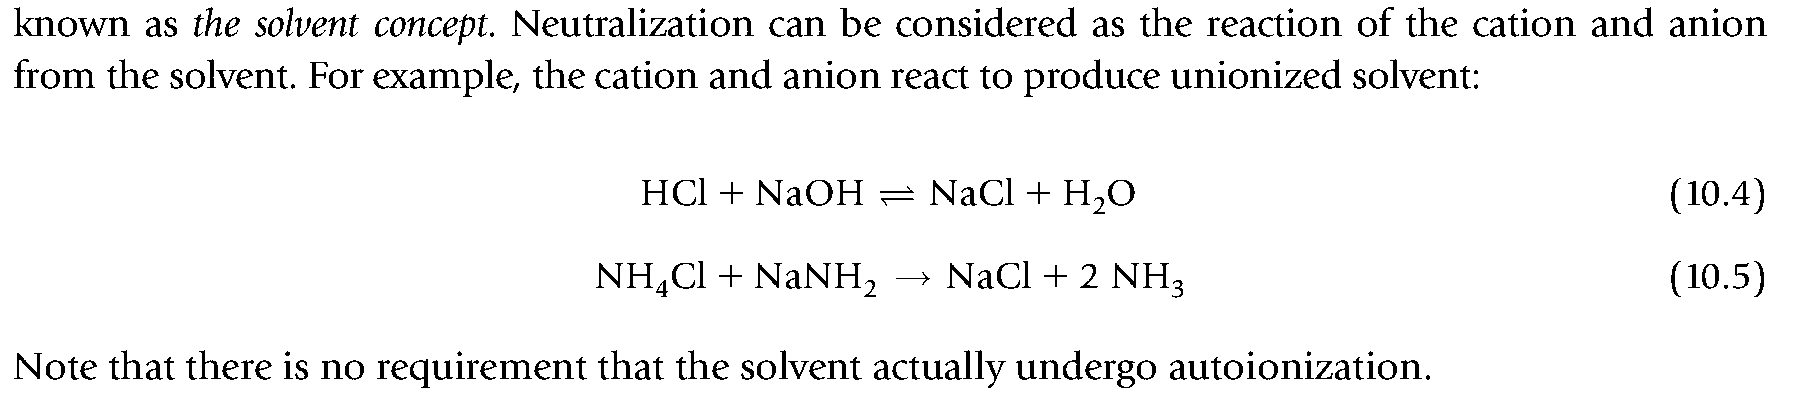
\includegraphics[width=0.35\textwidth]{simage.png} \\
 (a) Image\\ \hline
 \includegraphics[width=0.35\textwidth]{hproj.png} \\
 (b) Horizontal projection \\ \hline
 \end{tabular} 
 \caption{ A document page and its horizontal projection profile.}
 \label{H_PROJ}
\end{figure}
\subsubsection{Creation of word blobs}
\begin{figure}[h]\center\footnotesize
 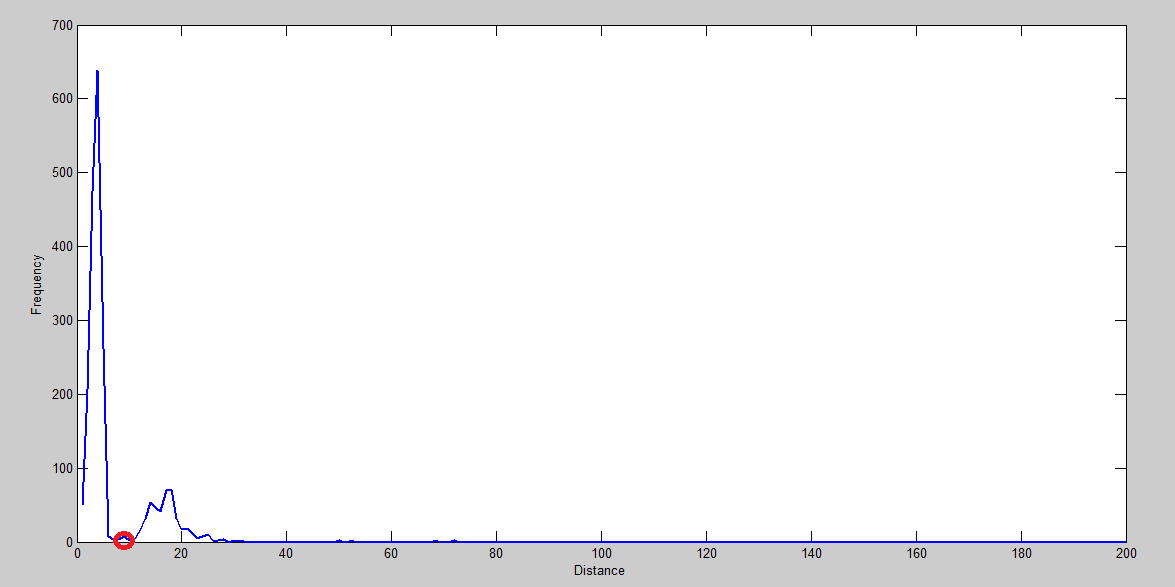
\includegraphics[width=0.35\textwidth]{histogram.png} 
   \caption{Distance histogram of the image shown in Fig.~\ref{H_PROJ} (a) }
 \label{hist}
\end{figure}

This is done by coalescing the characters in a word using morphological closing operation. Such character coalescing process depends on the accuracy in detecting 
the normal character gap and the gap between the consecutive connected components in  that text line. The component analysis is done first. Let $C_a$ and $C_b$ be the two  consecutive connected components in a text line. $L_b$ is the left most x coordinate of $C_b$ and $R_a$ is the right most x coordinate of $C_a$. A distance function $D$ is defined as follows:\\ $D = L_b - R_a$. The histogram of $D$ is obtained (see Fig.~\ref{hist}). The blob formation requires information on inter-word gap. The distance histogram is a multi-modal histogram. The first peak is corresponding to the character gaps. Our intention is to find out character gaps in running texts 
of a document page so that we could combine the consecutive characters into a single blob. Hence, we consider the upper boundary ($l$) of the first hump as the length of structuring element. Morphological close operation with a structuring element of size ($l\times 1$) will form the blobs. The result of blob formation is shown in Fig.~\ref{BLOB_FORM}.
\begin{figure}[h]\center\footnotesize
\begin{tabular}{|c|}
\hline
 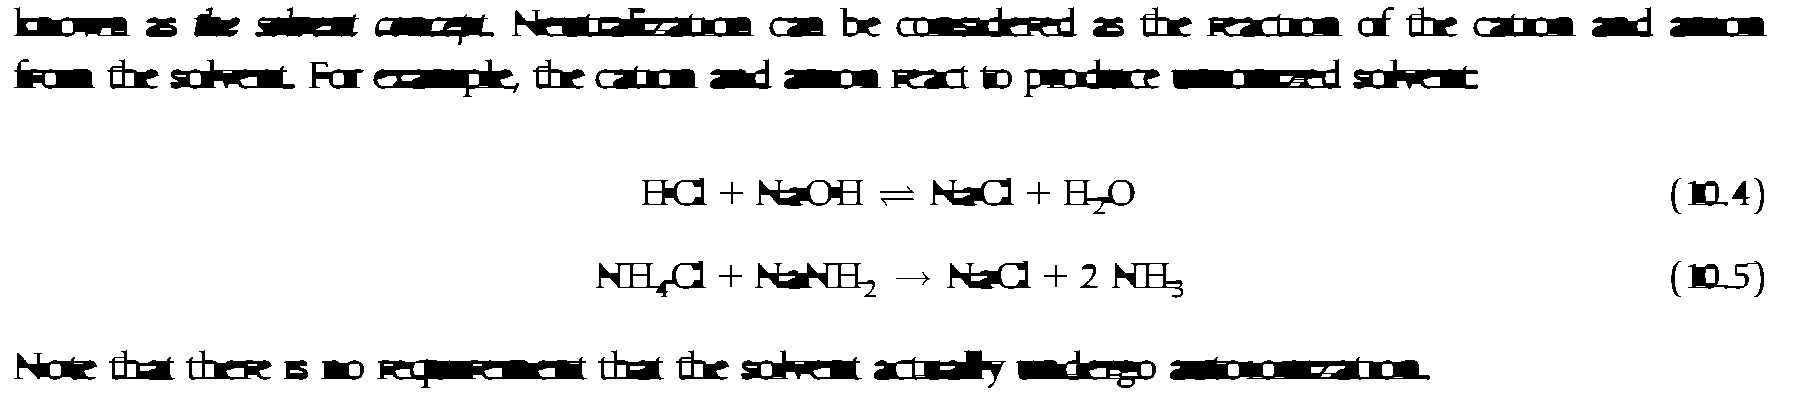
\includegraphics[width=0.35\textwidth]{blob.png} \\
 \hline
 \end{tabular} 
   \caption{Blob formation of the image shown in Fig.~\ref{H_PROJ} (a) }
 \label{BLOB_FORM}
\end{figure}

\subsubsection{DE zone extraction}
We have considered the set of operators that is commonly used both in chemical  equations as well as mathematical equations to fulfil our aim to classify displayed  zones containing chemical and non-chemical equations.

After blob formation, small component like dots of \emph{i and j} are  eliminated on the basis area. The region, corresponding to each blob  is considered from the original image and the number of connected component(s) present in that region is counted. If the number of components is more than one that blob is not an operator and is removed from the blob image (see Fig.~\ref{single_com}).
%Fig.~\ref{BLOB_FORM}.
\begin{figure}[h]\center\footnotesize
\begin{tabular}{|c|}
\hline
 \includegraphics[width=0.35\textwidth]{singlechar.png} \\
 \hline
 \end{tabular}
   \caption{Single components extracted from the blob image shown in Fig.~\ref{BLOB_FORM}}
 \label{single_com}
\end{figure}
The remaining components in the blob image are operators along with some alphanumerics like $‘a’$, $‘A’$, $‘(’$, etc. The logical AND operation is performed 
between the blob image and the original image. The Euler number of the operators  that we have considered is 1 (one) and based on this feature some of the alphanumerics are discarded. This image is denoted by  $I_s$. The components present in $I_s$ are divided into two classes; (i) one is operator class, and other is  non-operator class. We have considered the following operators (+,-,$\leftharpoondown$,$\rightharpoonup$,$\rightarrow$,$\leftrightarrow$) which are normally present in  chemical equations. \emph{One class} Support Vector Machine (SVM) classifier is trained to identify the operators from $I_s$. The features that we have used are as follows.
\begin{itemize}
 \item Aspect ratio ($f_a$) of each component
 \item 
 Density \[f_d   = \frac{\#pixels_o} {\#pixels_b}, \]
 where $\#pixels_o$ denotes the number of object pixels and $\#pixels_b$ denotes area of the bounding box.
 \item Each component is resized and horizontal and vertical projection profiles   are obtained.\\
 (i) For each profile the second ($f_{m2}$) and third moments ($f_{m3}$) are calculated. \\
 (ii) Again for each profile the location ($f_l$) and the magnitude ($f_m$) of the global maximum are determined.
 \item Perimeter ($f_p$)  of each component is also obtained.
\end{itemize}
The accuracy of the classifier is 98.4\%.

To detect `=' or `$\rightleftharpoons$' one extra step is required. 
The operators having $f_a$ $\leq$ 0.6 are considered  thin symbols (-,$\leftharpoondown$,$\rightharpoonup$,$\rightarrow$,$\leftrightarrow$). 
 For each symbol denoting thin operator, a rectangular mask is placed below the
symbol to check if there is another one within the mask. If  the two thin operators are present within the mask, they are considered  to form either
an `=' or `$\rightleftharpoons$' sign. Let the length of the thin operator be $l$. The area of the  mask is  ($l \times l/2$).

The horizontal line separating the numerator and the denominator is identified as its length is greater than the median length of the operators. Two windows are placed above and below the separating line to merge all the components within 
the windows with the separating line to form a single logical line. Otherwise, they  would be treated as three consecutive text lines and we will not be able to associate the intermediate math-symbols (‘+’, ‘-’, ‘=’) to a single expression. The  area of the window is (length of the separating line)$\times$ (twice the median width of the text lines).

Initially, all the text lines consisting at least one operator are considered  candidate displayed equations (CDE).
The operators are eliminated from CDE. The upper boundary ($u_v$) of the second hump of distance the histogram  is obtained which represents the word gaps in the text line. For each CDE zone Run Length Smoothing Algorithm  in horizontal direction (H-RLSA) is carried out. If the distance between two neighbouring components is less  than $u_v$, it means they belong to a same word and  are merged  by H-RLSA. H-RLSA has a similar effect as of dilation of black areas in horizontal  direction. The characters in a word are dilated and coalesced to the other characters of the same word. The output of H-RLSA is shown in Fig.~\ref{h-rlsa}.

Equation numbers are common in the displayed equation zones. These  numbers have to be removed because for each CDE we have counted the number of operators  and  corresponding other components  in the output of H-RLSA. If the number of components 
 $\le$ 2$\times$ number of operators, then the CDE is considered displayed equation;
 otherwise some embedded formulae/equations may exist in the line.
 To eliminate the equation number from the output of H-RLSA  the operators are  moved to the output of H-RLSA and the component 
analysis is done. From both ends distance ($d$) (see Fig. \ref{end_rev}) between the first two consecutive components is measured and if $d$  $> 5\times$  $u_v$, 
then the first component from the end is considered the  equation number and is removed. The accuracy of the DE zone segmentation is 97.4\%.

\subsection{Identification of chemical equations}
Each segment of a displayed equation is divided into three zones; namely upper zone, middle zone and lower zone (see Fig~\ref{sub_super}).
To identify the three zones of a DE zone, uppermost and lowermost co-ordinates of each connected component below the same DE zone  are also obtained.
The median of uppermost coordinate, and median of lowermost co-ordinate of such components in DE zone are computed.
A horizontal line, called the baseline, is drawn through the median of lowermost coordinates of components
and this baseline separates the middle zone and lower zone of DE zone.
Similarly, the median of uppermost co-ordinate of the components in the DE zone  generates a horizontal line. This horizontal line, called top line, separates the middle and  upper zones of the DE zone.

\begin{figure}[h]\center\
\begin{tabular}{|c|}
\hline
 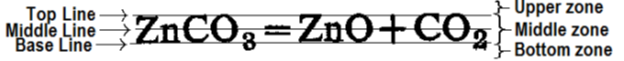
\includegraphics[width=0.42\textwidth]{supSub.png} \\ \hline
 \end{tabular} 
 \caption{Different zones of DE equation}
 \label{sub_super}
\end{figure}
The subscripts in a DE zone belong to lower-half of the middle zone and lower zone whereas the superscripts belong to upper zone and
upper-half of the middle zone. Based on the location of the components in a DE zone we have detected the subscripts and superscripts
and are separated from the DE zone. The operators are also separated from DE zone.
 
Now, each displayed equation is an input to an OCR of MATLAB R2014a.
The OCR returns each DE zone as a text string.
We made a dictionary out of all the elements in the periodic table. An important observation is that an element always starts with a capital letter. Using this property, an element can be expressed by a regular expression [A-Z][a-z]*. 
It means an element's symbol starts with an upper case letter and may or may not have lower case letters. 
We have designed a parser to extract the sub-string matching the regular expression  mentioned  above with the following grammar:
\begin{center}
$start \rightarrow capital.follow$\\
$follow \rightarrow small.follow | \in$\\
$capital \rightarrow A|B| \dots |X|Y|Z$\\
$small \rightarrow a|b| \dots |x|y|z$\\
\end{center}
Each of the substring returned by the parser is matched against the aforesaid dictionary and if it is a positive match then that substring is considered a symbol of the chemical element. 
Let us consider, the number of substrings extracted from the OCR output by the parser is {\em n}  and the number of positive matches 
the aforementioned dictionary is {\em m}.
If m:n ratio is more than a threshold value $\beta$ then this DE is considered  a Chemical Equation. 
This threshold ($\beta$) is set to 0.7 by running our algorithm on our dataset containing 985 displayed equations. The reason for the ratio not being 1 are (i)  Limitations of OCR; (ii) Touching and broken characters.



\section{Conclusions}
\label{conclude}
This paper presents a simple, but efficient binarization technique that can handle
 different types of degradation such as  faint characters, bleeding-through, large background
ink stains and the noise introduced in the scanning process (block noise) which are normally present at the border of images. 
We contend that the proposed method may be used as 'de facto' standard due to its simplicity and 
efficiency  for a variety of degraded images including
degraded handwritten historical documents.
%till it is replaced by a better one.
%\begin{figure}[h]\center\footnotesize
%\begin{tabular}{|c|}
%\hline \\
% \includegraphics[width=0.35\textwidth]{final_bi.png} \\ \hline
 %\end{tabular} 
 %\caption{Result after removal of isolated noise}
 %\label{final_img}
%\end{figure}
%The type II  noise generally appears at  the border of the  binarized image. It  may be characterised by the fact that the
%ratio of the  height and width  of the type II  noise component  is significantly larger than the ratio of the  height and width of the handwritten text. So,
%after the removal of type I noise, component analysis is done. Finally, the type II noise is eliminated  and on the basis of  ratio of the  height and width as
%indicated earlier.
% An example of a floating figure using the graphicx package.
% Note that \label must occur AFTER (or within) \caption.
% For figures, \caption should occur after the \includegraphics.
% Note that IEEEtran v1.7 and later has special internal code that
% is designed to preserve the operation of \label within \caption
% even when the captionsoff option is in effect. However, because
% of issues like this, it may be the safest practice to put all your
% \label just after \caption rather than within \caption{}.
%
% Reminder: the "draftcls" or "draftclsnofoot", not "draft", class
% option should be used if it is desired that the figures are to be
% displayed while in draft mode.
%
%\begin{figure}[!t]
%\centering
%\includegraphics[width=2.5in]{myfigure}
% where an .eps filename suffix will be assumed under latex, 
% and a .pdf suffix will be assumed for pdflatex; or what has been declared
% via \DeclareGraphicsExtensions.
%\caption{Simulation Results}
%\label{fig_sim}
%\end{figure}

% Note that IEEE typically puts floats only at the top, even when this
% results in a large percentage of a column being occupied by floats.


% An example of a double column floating figure using two subfigures.
% (The subfig.sty package must be loaded for this to work.)
% The subfigure \label commands are set within each subfloat command, the
% \label for the overall figure must come after \caption.
% \hfil must be used as a separator to get equal spacing.
% The subfigure.sty package works much the same way, except \subfigure is
% used instead of \subfloat.
%
%\begin{figure*}[!t]
%\centerline{\subfloat[Case I]\includegraphics[width=2.5in]{subfigcase1}%
%\label{fig_first_case}}
%\hfil
%\subfloat[Case II]{\includegraphics[width=2.5in]{subfigcase2}%
%\label{fig_second_case}}}
%\caption{Simulation results}
%\label{fig_sim}
%\end{figure*}
%
% Note that often IEEE papers with subfigures do not employ subfigure
% captions (using the optional argument to \subfloat), but instead will
% reference/describe all of them (a), (b), etc., within the main caption.


% An example of a floating table. Note that, for IEEE style tables, the 
% \caption command should come BEFORE the table. Table text will default to
% \footnotesize as IEEE normally uses this smaller font for tables.
% The \label must come after \caption as always.
%
%\begin{table}[!t]
%% increase table row spacing, adjust to taste
%\renewcommand{\arraystretch}{1.3}
% if using array.sty, it might be a good idea to tweak the value of
% \extrarowheight as needed to properly center the text within the cells
%\caption{An Example of a Table}
%\label{table_example}
%\centering
%% Some packages, such as MDW tools, offer better commands for making tables
%% than the plain LaTeX2e tabular which is used here.
%\begin{tabular}{|c||c|}
%\hline
%One & Two\\
%\hline
%Three & Four\\
%\hline
%\end{tabular}
%\end{table}


% Note that IEEE does not put floats in the very first column - or typically
% anywhere on the first page for that matter. Also, in-text middle ("here")
% positioning is not used. Most IEEE journals/conferences use top floats
% exclusively. Note that, LaTeX2e, unlike IEEE journals/conferences, places
% footnotes above bottom floats. This can be corrected via the \fnbelowfloat
% command of the stfloats package.

% trigger a \newpage just before the given reference
% number - used to balance the columns on the last page
% adjust value as needed - may need to be readjusted if
% the document is modified later
%\IEEEtriggeratref{8}
% The "triggered" command can be changed if desired:
%\IEEEtriggercmd{\enlargethispage{-5in}}

% references section

% can use a bibliography generated by BibTeX as a .bbl file
% BibTeX documentation can be easily obtained at:
% http://www.ctan.org/tex-archive/biblio/bibtex/contrib/doc/
% The IEEEtran BibTeX style support page is at:
% http://www.michaelshell.org/tex/ieeetran/bibtex/
%\bibliographystyle{IEEEtran}
% argument is your BibTeX string definitions and bibliography database(s)
%\bibliography{IEEEabrv,../bib/paper}
%
% <OR> manually copy in the resultant .bbl file
% set second argument of \begin to the number of references
% (used to reserve space for the reference number labels box)
\begin{thebibliography}{1}

%\bibitem{IEEEhowto:kopka}
%H.~Kopka and P.~W. Daly, \emph{A Guide to \LaTeX}, 3rd~ed.\hskip 1em plus
 % 0.5em minus 0.4em\relax Harlow, England: Addison-Wesley, 1999.
\bibitem{otsu_79}
 N.~Otsu, \emph{A threshold selection method from gray-level histograms},
Systems, Man and Cybernetics, IEEE Transactions, vol.9, no.1, pp. 62--66, 1979.

\bibitem{spc_07}
S.~P.~Chowdhury, S.~Mandal, A.~K.~Das, and B.~Chanda, \emph{Segmentation
of Text and Graphics from Document Images},
In Proc. of ICDAR, pp. 619–623,2007.

\bibitem{sekhar_06}
S.~Mandal, S.~P.~Chowdhury, A.~K.~Das, and B.~Chanda,
\emph{A simple and effective table detection system from Document Images},
IJDAR, Vol. 8(2), 172–182, 2006.

\bibitem{blostein_97}
D.~Blostein and A.~Grabavec,
\emph{Recognition of Mathematical Notation},
Handbook of Character Recognition and document Image Analysis,
577--582, 1997.
 
 \bibitem{chan_00}
K-F.~Chan and D-Y.~Yeung,
\emph{Mathematical Expression Recognition: A Survey},
IJDAR, Vol. 3, no: 1, 3–15, 2000.

\bibitem{Garain_07}
U.~Garain and B.~B.~Chaudhuri
\emph{On OCR of Printed mathematical Expressions, Digital Document Processing},
Ed: B.~B.~Chaudhuri, Advances in pattern Recognition, 235–259 , 2007.
 
\bibitem{uchid_10}
A.~Fujiyoshi, M.~Suzuki, S.~Uchid,
 \emph{Grammatical Verification for Mathematical Formula Recognition Based on Context-Free Tree Grammar},
 Mathematics in Computer Science, 279--298, 2010.
 
 
 \bibitem{algorri_07}
 M.~E.~Algorri, M.~Zimmermann, C.~M.~Friedrich, S.~Akle, and M.~Hofmann-Apitius,
\emph{Reconstruction of chemical molecules from images},
In Proc. 29th Annual International IEEE Conference on Engineering in
Medicine and Biology Society, 4609--4612, 2007.

\bibitem{algorri_07a}
M.~E.~Algorri, M.~Zimmermann, and M.~Hofmann-Apitius,
\emph{Automatic recognition of chemical images},
In pro. Eighth Mexican International Conference on Current Trends in Computer Science, 41--46, 2007.
\bibitem{park_09}
J.~Park, G.~R.~Rosania, K.~A.~Shedden, M.~Nguyen, N.~Lyu, and K.~Saitou,
\emph{Automated extraction of chemical structure information from digital raster images}, Chemistry Central journal, vol. 3(1), 2009.
%
%\bibitem{lu_10}
% S.~Lu, B.~Su,  C.~L.~Tan,
%\emph{ Document image binarization using background estimation and stroke edges},
% IJDAR, vol. 13, no. 4, pp.303--314, 2010.
% 
% %\bibitem{lu_10a}
%%S.~Lu, B.~Su,  C.~L.~Tan,
%%\emph{Binarization of Historical Document Images Using The Local Maximum and Minimum},
%%Proc. Intl. Workshop on Document Analysis Systems, pp.159--165, 2010.
%
%\bibitem{kim_02}
%Kim,~I.~K., Jung,~D.~W., Park,~R.~H,
%\emph{Document image binarization based on topographic analysis using a water flow model},
% Pattern Recognition vol. 35, no. 1, pp.265--277, 2002.
% 
% \bibitem{kuk_09}
%J.~G.~Kuk and N.~I.~Cho,
%\emph{Feature based binarization of document images degraded by uneven light condition},
% In Proc. ICDAR, pp. 748--752, 2009.
% 
% \bibitem{le_11}
%T.~Le, T.~Bui, and C.~Suen,
%\emph{Ternary entropy-based binarization of degraded document images using morphological operators},
% In Proc. ICDAR, pp. 114--118, 2011.
% 
% \bibitem{kan_09}
%T.~Li-Jing, C.~Kan, Z.~Yan, F~ Xiao-ling, and D.~Jian-Yong,
%\emph{Document image binarization based on nfcm},
%In Proc. Image and Signal Processing, pp. 1--5, 2009.
%
%\bibitem{gatos_12}
%K.~Ntirogiannis, B.~Gatos and I.~Pratikakis,
%\emph{A combined approach for the binarization of handwritten document images},
%Pattern Recognition Letters vol. 35, pp.3--15, 2012.
%
%\bibitem{gatos_09}
% B.~Gatos, K.~Ntirogiannis and I.~Pratikakis,
%\emph{ICDAR 2009 document image binarization contest (DIBCO 2009)},
%In Proc. ICDAR, pp.1375--1382, 2009.
%
%\bibitem{lu_04}
%Lu.~H,  A.~C.~Kot and Y.~Q.~Shi.
%\emph{Distance-Reciprocal Distortion Measure for Binary Document Images},
%IEEE Signal Processing Letters, vol. 11, No. 2, pp. 228--231, 2004.
%
%\bibitem{su13}
%B.~Su, S.~Lu,  C.~L.~Tan.
%\emph{A Robust Document Image Binarization for Degraded Document Images},
%IEEE Transactions on Image Processing, vol.22, no. 4, pp. 1408--1417, April 2013. 
%

%\bibitem{gonzalez_92}
 %R.~C.~Gonzalez and R.~Wood,
%\emph{Digital Image Processing},
%\Addision-Wesley, 1992.






\end{thebibliography}




% that's all folks
\end{document}

